\documentclass[a4paper,12pt,reqno]{amsart}
\usepackage{M67tds}

% pour voir les solutions il faut enlever le commentaire de la ligne suivante
\solutionstrue

% Les notes de bas de page dans les minipages (sidebyside)
\renewcommand{\thempfootnote}{\fnsymbol{mpfootnote}}

% pour surligner
\sisolutions{
  \usepackage{soul}
  \colorlet{hl}{yellow!35!white}
  \sethlcolor{hl}
}

\begin{document}

% ==================================
\hautdepage{

\ifsolutions{Solutions de l'examen}\else{Examen final}\fi\par\normalfont\normalsize
17 mai 2018\\{[ durée: 3 heures ]}\par
}
% ==================================
\ifsolutions\else
% {\fontencoding{U}\fontfamily{futs}\selectfont\char 66\relax}
\tikz[baseline=(e.base)]{\NoAutoSpacing\node(e){!};\draw[red,ultra thick,line join=round,yshift=-.15ex](90:1em)--(210:1em)--(330:1em)--cycle;}
\textbf{Documents autorisés :}\textit{Une feuille A4 recto-verso écrite à la main.}

\vspace{7mm}
% \tsvp
\fi

%-----------------------------------
\begin{exo}

  Soit $ABCD$  un trapèze convexe de bases $[AB]$ et $[CD]$ \emph{(c.-à-d. tel que $(AB)$ et $(CD)$ sont parallèles)}. Soient $O$ le point d'intersection de $[AC]$ et $[BD]$, $\Delta$ la parallèle à $(AB)$ passant par $O$, et $I$ (resp. $J$) le point d'intersection de $\Delta$ et $[AD]$ (resp. de $\Delta$ et $[BC]$).
  \begin{enumerate}
    \item Montrer que $IO=\dfrac{AB \cdot CD}{AB+CD}$.\quad
    \begin{indication}
      Utiliser deux fois Thalès.
    \end{indication}
    \item Exprimer $IJ$ en fonction de $AB$ et $CD$.
  \end{enumerate}
\end{exo}

\begin{solution}
  \begin{enumerate}
    \item
      \sidebyside{.7}{
        Puisque $(OI)$ et $(DC)$ sont parallèles, le théorème de Thalès dans le triangle $\tri ACD$ assure que $IO:DC=AI:AD$, et le même théorème dans $\tri ABD$ assure que $IO:AB=ID:AD$. Puisque $I$ est entre $A$ et $D$ on obtient en ajoutant ces deux égalités
        $$
          \frac{IO}{CD}+\frac{IO}{AB}=\frac{AI+ID}{AD}=1,
        $$
        d'où le résultat attendu.
      }{\hfill
        \raisebox{-\height}[0pt][0pt]{
          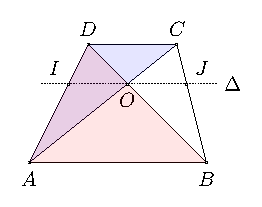
\includegraphics[width=4cm]{M67_2017-18_DS2_img_exo1sol}
        }
      }
    \item On a de même $OJ=\dfrac{AB \cdot CD}{AB+CD}$, puis $IJ=IO+OJ=2\dfrac{AB \cdot CD}{AB+CD}$.
  \end{enumerate}
\end{solution}

%-----------------------------------
\begin{exo} (Théorème de Viviani)

  Soit $ABC$ un triangle équilatéral. Soit $M$ un point intérieur au triangle $ABC$. Montrer que la somme des distances du point $M$ aux trois côtés du triangle est égale à la hauteur de ce triangle.
\end{exo}

\begin{solution}
  \sidebyside{.7}{
    On note $a$ et $h$ respéctivement la longueur du côté et la hauteur du triangle équilatéral $\tri ABC$. Soient $I$, $J$ et $K$ les projetés orthogonaux de $M$ sur respectivement $[BC]$, $[AC]$ et $[AB]$. Le triangle $ABC$ est alors réunion des trois triangles $\tri BMC$, $\tri AMC$ et $\tri AMB$, dont les aires valent respectivement $\frac{1}{2} BC \cdot MI$, $\frac{1}{2} CA \cdot MJ$ et $\frac{1}{2} AB \cdot MK$. Comme les intersections de ces triangles sont des segments, l'aire $\frac{1}{2}ah$ du trangle $\tri ABC$ est la somme de leurs trois aires. Ainsi $\frac{1}{2}a(MI+MJ+MK) = \frac{1}{2}ah$, et on en déduit que la somme $MI+MJ+MK$ des distances de $M$ aux trois côtés est égale à l hauteur $h$ du triangle $\tri ABC$.
  }{\hfill
    \raisebox{-\height}[0pt][0pt]{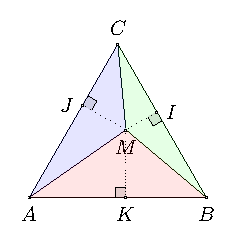
\includegraphics[width=4cm]{M67_2017-18_DS2_img_exo2sol}}
  }
\end{solution}

%------------------------------------
\begin{exo} (CAPES 2011 - Construction de triangles)

 Dans le plan affine euclidien orienté, on considère deux points distincts $B$ et $C$ et un point $M$ en dehors de la droite $(BC)$.

 Pour chacune des assertions suivantes, déterminer s'il existe un point $A$ qui la vérifie. On précisera dans chaque cas le nombre de solutions et on prendra soin de fournir toutes les explications et justifications utiles.
   \begin{enumerate}
    \item $M$ est le centre de gravité du triangle $ABC$.
    \item $M$ est le centre du cercle circonscrit au triangle $ABC$.
    \item $M$ est l'orthocentre du triangle $ABC$.
    \item $M$ est le centre du cercle inscrit dans le triangle $ABC$.
   \end{enumerate}
\end{exo}

\begin{solution}
  \begin{enumerate}
    \item
      \sidebyside{.7}{
        Rappelons que, si $I$ est le milieu de $[BC]$, le centre de gravité $M$ d'un triangle $ABC$ est le point de $[IA]$ tel que $IM=\frac{1}{3} IA$. Il existe donc un unique point $A$ tel que $M$ soit le centre de gravité de $ABC$, et c'est l'unique point de la demi-droite $[IM)$ tel que $IA=3 IM$.
      }{\hfill
        \raisebox{-.7\height}[0pt][0pt]{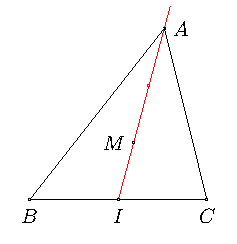
\includegraphics[width=35mm]{M67_2017-18_DS2_img_exo3asol}}
      }
    \item
      \sidebyside{.7}{
        Le centre du cercle circonscrit à un triangle est l'unique point à égale distance des sommets $A$, $B$ et $C$. Ainsi, si $MB \neq MC$ il n'existe aucun point $A$ tel que $M$ soit le centre du cercle circonscrit à $\tri ABC$. En revanche, si $MB=MC$, alors, pour tout point $A$ du cercle de centre $M$ passant par $B$, distinct de $B$ et $C$, le centre du cercle circonscrit à $ABC$ est $M$.
      }{\hfill
        \raisebox{-.84\height}[0pt][0pt]{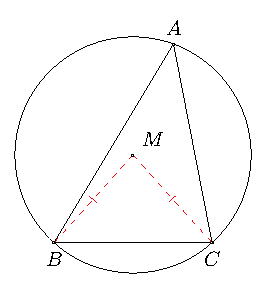
\includegraphics[width=35mm]{M67_2017-18_DS2_img_exo3bsol}}
      }
    \item
      \sidebyside{.7}{
        Remarquons que si $BI$ et $CJ$ sont des hauteurs dans $\tri ABC$ (voir image), alors $CI$ et $BJ$ sont des hauteurs dans $\tri MBC$. Ainsi $M$ est l'orthocentre de $\tri ABC$ si et seulement si $A$ est l'orthocentre de $\tri BCM$. Il existe ainsi une unique point $A$ tel que $M$ soit l'orthocentre de $\tri ABC$, et c'est l'orthocentre de $\tri BCM$.
      }{\hfill
        \raisebox{-.84\height}[0pt][0pt]{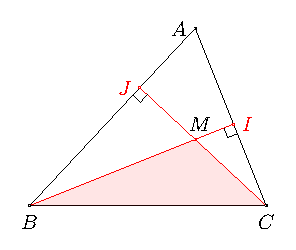
\includegraphics[width=35mm]{M67_2017-18_DS2_img_exo3csol}}
      }
    \item
      \sidebyside{.7}{
        Si $M$ est le centre du cercle inscrit dans $ABC$, alors $\widehat{ABC}=2\widehat{MBC}$ et $\widehat{ACB}=2\widehat{MCB}$, de sorte que $A$ est le point d'intersection de deux demi-droites uniquement déterminées par $B$, $C$ et $M$. Ces deux demi-droites se coupent si et seulement si $\widehat{MBC} + \widehat{MCB} < \pi/2$ \emph{(c.-à-d. si et seulement si $\tri CMB$ est obtus en $M$)}.
      }{\hfill
        \raisebox{-\height}[0pt][0pt]{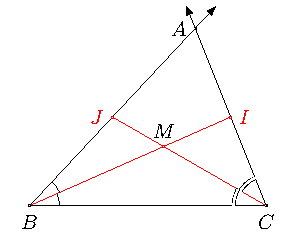
\includegraphics[width=35mm]{M67_2017-18_DS2_img_exo3dsol}}
      }
  \end{enumerate}

\end{solution}


%-----------------------------------
\begin{exo}

  Soit $ABC$ un triangle. Soit $P$ un  point  du segment $[BC]$. On note $M$ (resp. $N$) son projeté orthogonal sur $(AB)$ (resp. sur $(AC)$). On cherche $P$ tel que la distance $MN$ soit minimale.
  \begin{enumerate}
    \item Étudier le cas d'un triangle $ABC$ rectangle en $A$.
    \item On suppose maintenant $ABC$ quelconque.
    \begin{enumerate}
      \item Montrer que $\dfrac{MN}{AP}=\sin{\widehat{BAC}}$.
      \item Conclure.
    \end{enumerate}
  \end{enumerate}

\end{exo}

\begin{solution}
  \begin{enumerate}
    \item
      \sidebyside{.7}{
        Si l'angle en $A$ est droit, alors $AMPN$ est un parallélogramme avec un angle droit, donc un rectangle, et ses diagonales $AP$ et $MN$ sont égales. Minimiser $MN$ revient donc à minimiser $AP$. Or, lorsque $P$ parcourt la droite $(BC)$, $AP$ est minimale lorsque $P$ est le projeté orthogonal $A'$ de $A$ sur $(BC)$.
        Comme le triangle $\tri ABC$ n'est pas obtus, tout les pieds des hauteurs sont sur les côtés du triangle, donc en particulier $A' \in [BC]$ est la position recherchée de $P$.
      }{\centering
        \raisebox{-\height}[0pt][0pt]{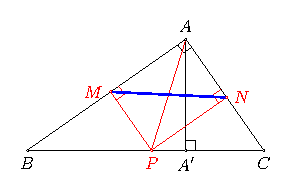
\includegraphics[width=49mm]{M67_2017-18_DS2_img_exo4asol}}
      }
    \item
      \begin{enumerate}
        \item
          \sidebyside{.7}{
            Soit $\alpha$ la mesure de l'angle $\widehat{BAC}$. Puisque les triangles $AMP$ et $ANP$ sont rectangles en $M$ et $N$, les points $M$ et $N$ appartiennent au cercle de diamètre $[AP]$ et les angles $\widehat{MPN}$ et $\widehat{MAN}$, qui éclairent la corde $MN$, on le même sinus, $\sin \alpha$. La longueur de la corde $[MN]$ vaut alors $AP\sin\alpha$. Cette formule reste vrai même dans les cas limites où deux des points $M$,$N$,$A$ et $P$ coïncident.
          }{\centering
            \raisebox{-\height}[0pt][0pt]{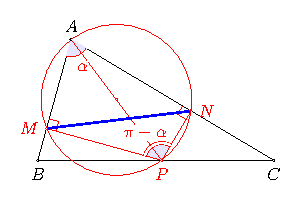
\includegraphics[width=49mm]{M67_2017-18_DS2_img_exo4bsol}}
          }
        \item Alors à nouveau $MN$ est minimale quand $AP$ l'est. Si $A' \in [BC]$ alors $P=A'$ est la position recherché, comme dans la question précédente, si $B \in [A'C]$ alors $P=B$ et dans le dernier cas, $C \in [BA']$, c'est $P=C$ est la position recherché.
      \end{enumerate}
  \end{enumerate}

\end{solution}

%-----------------------------------
\begin{exo} (Kangourou 2006)

  \sidebyside{.7}{
    On considère la figure ci-contre ; le quotient du rayon du secteur circulaire par le rayon du cercle inscrit dans ce secteur est 3. Quel est le quotient des aires de ce secteur circulaire et du cercle inscrit ?
  }{
    \raisebox{-.7\height}[0pt][0pt]{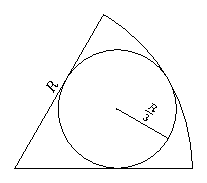
\includegraphics[width=4cm]{img_kangourou2006}}
  }
\end{exo}

\begin{solution}
  \sidebyside{.7}{
    On note les points comme sur la figure ci-contre. Comme $O_{1}O_{2}=R-\frac{1}{3}R = \frac{2}{3}R$, on trouve que $\widehat{O_{2}O_{1}Q} = \arctan \frac{O_{2}Q}{O_{1}O_{2}}=\arctan \frac{1}{2}=30^{\circ}$. Ainsi l'aire du secteur est $\frac{1}{6}\pi R^{2}$ et l'aire du disque est $\frac{1}{9}\pi R^{2}$. Donc le rapport recherché est $\frac{3}{2}$.
  }{
    \raisebox{-.7\height}[0pt][0pt]{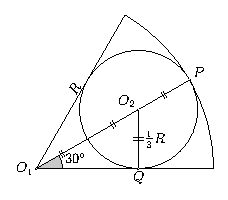
\includegraphics[width=4cm]{img_kangourou2006b}}
  }
\end{solution}



\end{document}
